\chapter{Setting up an Arduino on a breadboard}

This tutorial shows you how to build an Arduino compatible breadboard with an Atmel Atmega8/168 AVR microcontroller and FTDI FT232 breakout board from SparkFun.
Originally created by Carlyn Maw
Updated October 23, 2008 by Rory Nugent

To do this, you'll need:

The Supplies

\subsection{Basic Parts for wiring up Arduino}

A breadboard
22 AWG wire
7805 Voltage regulator
2 LEDs
2 220 Ohm resistors
1 10k Ohm resistor
2 10 uF capacitors
16 MHz clock crystal
2 22 pF capacitors
small momentary normally open ("off") button, i.e. Omron type B3F

\subsection{USB to Serial Communication Board}

You will need a FT232 USB Breakout board from SparkFun.
There are two options available from them:
FT232RL USB to Serial Breakout Board, SKU BOB-0071
Arduino Serial USB Board, SKU DEV-08165
If you plan to use the top option and have not yet soldered headers to the breakout board, now would be a good time.
1.3  Bootloading your Atmega Chips (Optional)

There are several options for bootloading your Atmega chips, a few of which are covered in this tutorial. If you wish to bootload your Atmega chips using your breadboard, an additional part will make your life much easier but is not necessary.
AVR Programming Adapter from Sparkfun, SKU BOB-08508

\section{Adding circuitry for a power supply}

If you've already worked with microcontrollers, it is likely that you already have a preferred way to wire up a power supply to your board, so go ahead and do it that way. In case you need some reminders, here are some pictures of one way to go about it. (We are going for a 5V regulated power supply)


Top Power lines
Add power and ground wires for where your voltage regulator will be. 


Bottom Power lines
Add power and ground wires at the bottom of your board connecting each rail. 


Add the 7805 and decoupling capacitors
Add the 7805 power regulator and the lines to power the board. The regulator is a TO-220 package where the IN-line from the external power supply goes IN on the left, ground is in the middle and the 5V OUT is on the right (when facing the front of the regulator). We're also adding power OUT and ground wires that connect to the right rail and power IN and ground wires off to the left where our power supply may go.
Also, add a 10uF capacitor between the IN of the regulator and the ground as well as a 10uF capacitor on the right rail between power and ground. The silver strip on the capacitor signifies the ground leg.


LED
Add an LED on the left side of your board across from the voltage regulator. An LED attached to power like this is a great troubleshooting trick. You'll always know when your board is being powered as well as quickly know if your board is being shorted. 

Power Supply Input
The red and black wires to the left of the voltage regulator is where your power supply will be plugged in. The red wire is for the POWER and the black wire is for the GROUND. Be sure to only attach a power supply that is between 7-16V. Any lower and you won't get 5V out of your regulator. Any higher and your regulator may get too hot. A 9V battery, 9V DC power supply, or 12V DC power supply is suitable. 

Blank Canvas
Now that the power-basics are done we are ready to load on the chip!

\section{ATMEGA8/168 Basics}


Arduino Pin Map
Before moving on, this image is a great resource for learning what each of the pins on your Atmega chip do in relation to the Arduino's functions. This will clarify a lot of confusion behind why we hook up certain pins the way we do. For even more detailed information, take a peek at the datasheet for the Atmega 168 (short version) (long version).


Add supporting circuitry
Start by adding a 10k ohm resistor "up" (to power) on the RESET pin in order to prevent the chip from resetting itself during normal operation. The RESET pin reboots the chip when pulled down to ground. In later steps we will show you how to add a reset switch that takes advantage of this.
Pin 7 - Vcc - Digital Supply Voltage
Pin 8 - GND
Pin 22 - GND
Pin 21 - AREF - Analog reference pin for ADC
Pin 20 - AVcc - Suppply voltage for the ADC converter. Needs to be connected to power if ADC isn't being used and to power via a low-pass filter if it is (a low pass filter is a circuit that cleans out noise from the power source, we aren't using one)


Add the Clock \& Caps
Add a 16 MHz external clock between pin 9 and 10, and add two 22 pF capacitors running to ground on each of those pins.


Add a reset switch
This is where we add the small tactile switch so that we can reset the Arduino whenever we'd like and prepare the chip for uploading a new program. A quick momentary press of this switch will reset the chip when needed. Add the switch just above the top of the Atmega chip crossing the gap in the breadboard. Then, add a wire from the bottom left leg of the switch to the RESET pin of the Atmega chip and a wire from the top left leg of the switch to ground.


LED leads on Arduino pin 13
The chip I'm using on this board is actually already programmed using the blin\_led program that comes with the Arduino software. If you already have an Arduino printed circuit board running it is a good idea to go ahead and check the breadboard version you are building with a chip you know works. The blink\_led program blinks pin 13. Pin 13 on the Arduino is NOT the AVR ATMEGA8-16PU/ATMEGA168-16PU pin 13. It is actually pin 19 on the Atmega chip.
Refer to the pin mapping above to be sure you are plugging it in correctly.


LED on Arduino Pin 13
Finally, add the LED. The long leg or the cathode connects to the red wire and the short leg or the anode connects to the 220 ohm resistor going to ground.


Arduino-Ready!
At this point if you had already programmed your chip somewhere else and didn't need this breadboard circuit to reprogram the chip, you could stop here. But part of the fun is in-circuit programming so keep going to really make a full USB-Arduino-circuit on a breadboard!

\section{Arduino-Ready}


Add FT232 USB to Serial Board
Now we'll be adding the USB to Serial breakout board to our Arduino breadboard circuit. If you haven't added male headers to your breakout board, you will need to do it now.
Connect pin 6 of the breakout board to power and pin 9 to ground. With the USB port facing upward, I'm calling the top left pin 1, the bottom left 9, the top right 10, and the bottom right 18.


The pinouts of the Sparkfun FT232 breakout
Curious what all the pin outs are for the SparkFun FT232 breakout board, just simply flip it over! In this situation we'll be using VCC (to supply 5V from the USB port to your board), GND, TXD, and RXD.


Connecting the TX and RX
Now, let's get the USB to serial breakout board talking with your new Arduino setup. Connect the RX (pin 2) of your Atmega chip to pin 10 of the USB to serial board, and connect the TX (pin 3) of your Atmega chip to pin 14 of the USB to serial board.

And there you have it... ready to be plugged in, powered up and programmed!
But wait, there's another step right? If you pulled your Atmega chip out of your Arduino, it has most likely been programed several times by yourself and so it definitely has been bootloaded, so you won't need to move any further in this tutorial.
However, if you purchased some extra Atmega8 or Atmega168 chips from an online store they will have NOT been bootloaded with the Arduino bootloader (with the exception of Adafruit Industries). What does this mean? You won't be able to program your chips using the USB to serial breakout board and the Arduino software. So, in order to make your new chips useful for Arduino you MUST bootload them and MUST check out step 4.

\section{Other Breadboard Options}

The uDuino Setup by Tymn Twillman
This configuration is similar to the one above but the trick is that the Atmega chip is bootloaded with the Arduino Lilypad bootloader. The Lilypad runs using the internal clock instead of an external clock and so removes the need for much of the supporting circuitry.
Boarduino by Ladyada
The Boarduino is a kit you purchase and assemble to create a nice, small breadboard compatible Arduino set up. All the common components are included on a small PCB so that the Boarduino can easily be added to a breadboard and even removed, in a snap.

\section{Bootloading your chips OPTIONAL}

\subsection{Bootloading Options}

There are two options for bootloading your chips. The first being quite easy and the other being a little more tricky. We will cover both.
Bootloading your Atmega chip using a Arduino board and an AVR programmer
Bootloading your Atmega chip in your newly prepared breadboard with an AVR programmer
There are also many different kinds of AVR programmers but two are most commonly used here at ITP:

AVRISP mkII

USBtinyISP

The AVRISP mkII can be found in the ER or can be purchased from Digikey (Part \# ATAVRISP2-ND) while the USBtinyISP must be assembled and can be found at Adafruit Industries.

\subsection{Using an Arduino board}


Bootloading on an Arduino board
Place your Atmega chip into the Arduino board with the divot of the chip facing outward. Set the jumper to an external power supply and connect a 12V power brick (your board needs to be externally powered when using the AVR ISP mkII but is not needed with the AVRtinyISP) . Then, attach the 6-pin female plug of your AVR programmer to the 6 male header ICSP pins with the plastic nub of the ribbon cable head facing inward.
NOTE: The AVR ISP mkII turns its LED green when they've been hooked up correctly and are ready for programming. The LED turns red if it is hooked up wrong.

\subsection{Using your breadboard}


AVR Programming Adapter
When bootloading an Atmega chip on a breadboard, I found the AVR programming adapter (SKU BOB-08508) from Sparkfun to be incredibly handy. This adapter breaks out the 6 pins from the programmer to 6 inline pins for easy attachment to the breadboard. All the pins are also labeled making it very easy to connect it up to your chip.


6-pin AVR Programmer Cable
Don't worry, if you don't have an AVR programming adapter you can still bootload without it. It will however be more of a headache to set up. The two images to the left are great references when hooking up a programmer to an Atmega chip without an adapter board. The images will tell you what all the holes in the 6-pin AVR plug are and you will simply need to stick wires in the end and run them to your Atmega chip.


6-pin AVR Programmer Cable Head
This image is a view from the bottom and labels each of the holes. Take note of the square as to what orientation your cable is in.


Add power and ground
Let's begin!
With the breadboard you prepared above, add two wires for power and ground for your AVR programmer.


Plug in the AVR adapter
Now plug the AVR programming adapter into the breadboard with the GND pin matching up with the ground wire you just ran and the 5V pin matching up with the power wire you just ran.


Add the MISO, SCK, RESET, and MOSI wires
In this step you will need to add the last four wires needed by the AVR programmer for proper bootloading.
Be sure to refer to the Arduino pin mapping for help wiring this up.
The MISO pin of your adapter will go to pin 18 or Arduino digital pin 12 of your Atmega chip.
The SCK pin of your adapter will go to pin 19 or Arduino digital pin 13 of your Atmega chip.
The RESET pin of your adapter will go to pin 1 of your Atmega chip.
The MOSI pin of your adapter will go to pin 17 or Arduino digital pin 11 of your Atmega chip.


Plug in the USB cable and AVR programming cable
Almost there! Just plug in a USB cable to your USB breakout board and plug the 6-pin plug of your AVR programmer to your AVR programming adapter. The black nub of the 6-pin head must be facing upwards towards the Atmega chip.
In the next step, we'll show you have to use the Arduino software to burn your bootloader!

\subsection{Time to burn!}


Pick your board type
Fire up Arduino and then go to 'Tools' and 'Board'. Choosing the type of board you'd like to use will effect which bootloader you will be put on your chip. Most commonly you will be using the Diecimilia or the most recent version of Arduino for an Atmega PDIP, however if you'd like to bootload an Arduino Lilypad, Arduino Mini, Arduino Nano, or any of the older Arduino versions, choose the appropriate board.


Choose your programmer. Burn!
Then, go to 'Tools' and 'Burn Bootloader' and choose the programmer you will be using.


Burning
Once you chose your programmer, the AVR programmer will begin bootloading your Atmega chip and a message will appear in the status bar which reads "Burning bootloader to I/O Board (this may take a minute)..." Lights will flicker on your programmer.


Burn Complete!
When done bootloading, the status bar will be updated with the message "Done burning bootloader." Your chip is now ready to be programmer using the Arduino software! Congrats! Power cycle your Arduino and your new Atmega chip will be running a simple LED blink program with pin 13 (if this is not the case, try programming it with one). If this is working, it was most definitely a success.

NOTE: On occasion, the process of bootloading an Atmega chip with the AVR ISP mkII will take an extraordinarily long period of time. Usually it should only take a couple minutes and in fact, the AVRtinyISP finishes much quicker. However, there are times where after 5-10 minutes it still appears to be bootloading. I found this to be an odd hiccup (perhaps it is triple checking the data flow) and after giving it ample time, 10 minutes or so, I usually unplug the programmer only to find the burning process to be a success and has ended long ago. I by no means endorse this method and you take all responsibility in whatever may happen to your chip, but in my experience it has been fairly harmless though you should proceed with caution. It is very possible that you may damage your chip in the process.

\begin{figure}[!htb]
 \centering
 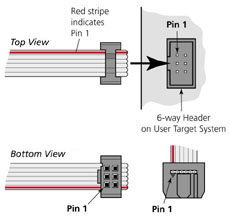
\includegraphics[scale=0.3]{img/arduino_breadboard/6pinAVRprogcable.jpg}
 \caption{6pinAVRprogcable}
 \label{6pinAVRprogcable}
\end{figure}


\begin{figure}[!htb]
 \centering
 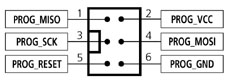
\includegraphics[scale=0.3]{img/arduino_breadboard/6pinAVRproghead.jpg}
 \caption{6pinAVRproghead}
 \label{6pinAVRproghead}
\end{figure}


\begin{figure}[!htb]
 \centering
 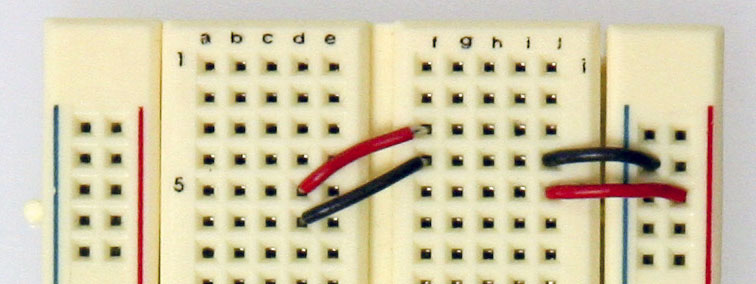
\includegraphics[scale=0.3]{img/arduino_breadboard/arduinobb_02.jpg}
 \caption{arduinobb 02}
 \label{arduinobb 02}
\end{figure}


\begin{figure}[!htb]
 \centering
 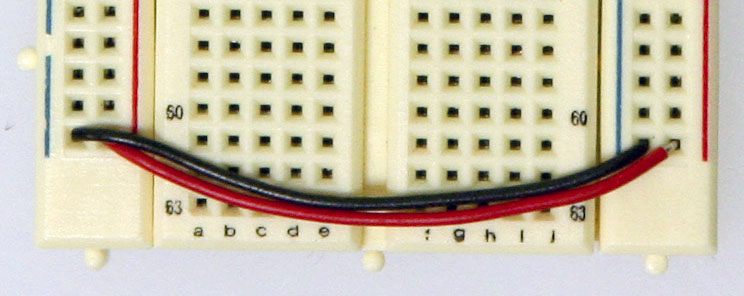
\includegraphics[scale=0.3]{img/arduino_breadboard/arduinobb_03.jpg}
 \caption{arduinobb 03}
 \label{arduinobb 03}
\end{figure}


\begin{figure}[!htb]
 \centering
 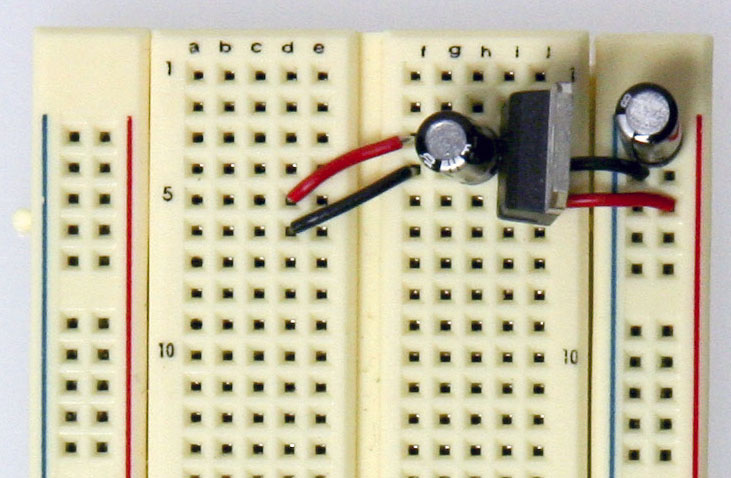
\includegraphics[scale=0.3]{img/arduino_breadboard/arduinobb_04.jpg}
 \caption{arduinobb 04}
 \label{arduinobb 04}
\end{figure}


\begin{figure}[!htb]
 \centering
 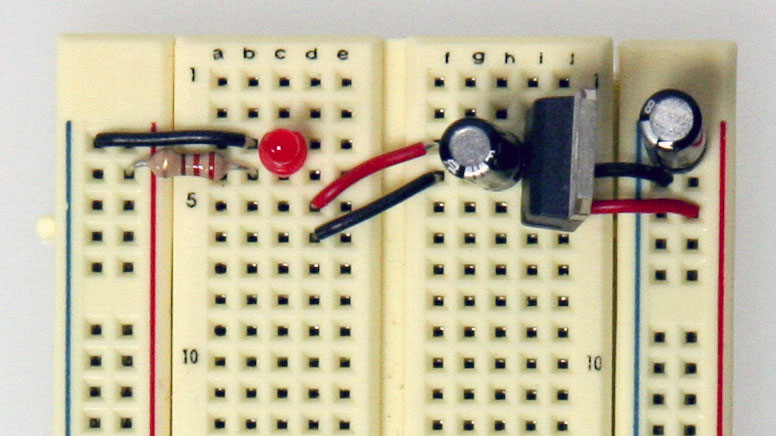
\includegraphics[scale=0.3]{img/arduino_breadboard/arduinobb_05.jpg}
 \caption{arduinobb 05}
 \label{arduinobb 05}
\end{figure}


\begin{figure}[!htb]
 \centering
 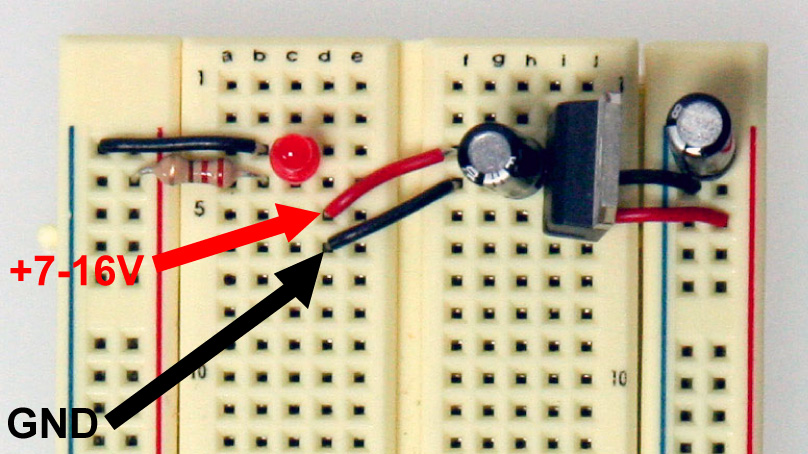
\includegraphics[scale=0.3]{img/arduino_breadboard/arduinobb_05_supply.jpg}
 \caption{arduinobb 05 supply}
 \label{arduinobb 05 supply}
\end{figure}


\begin{figure}[!htb]
 \centering
 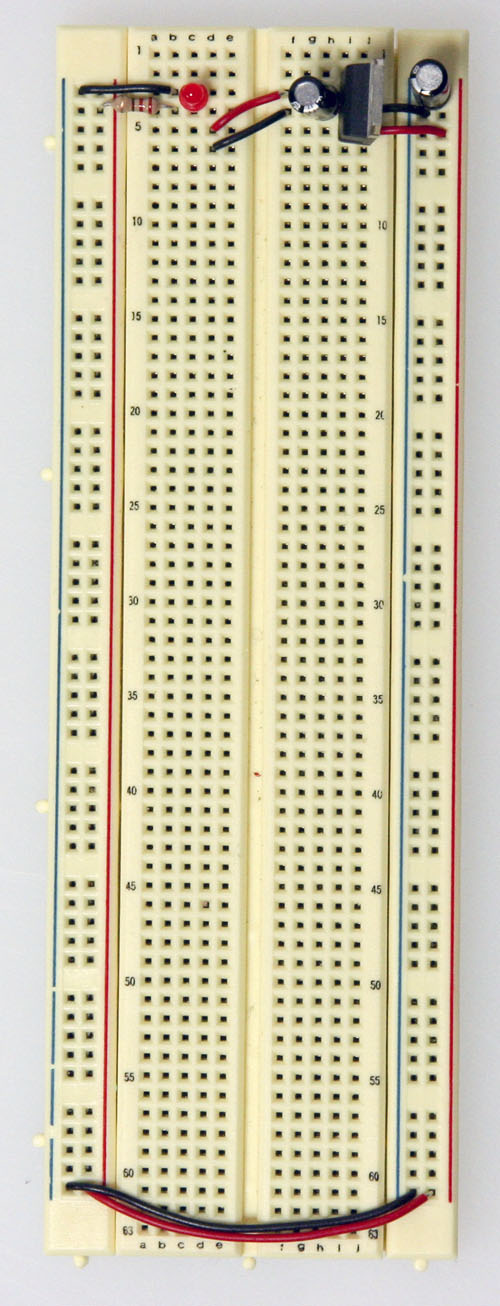
\includegraphics[scale=0.3]{img/arduino_breadboard/arduinobb_06.jpg}
 \caption{arduinobb 06}
 \label{arduinobb 06}
\end{figure}


\begin{figure}[!htb]
 \centering
 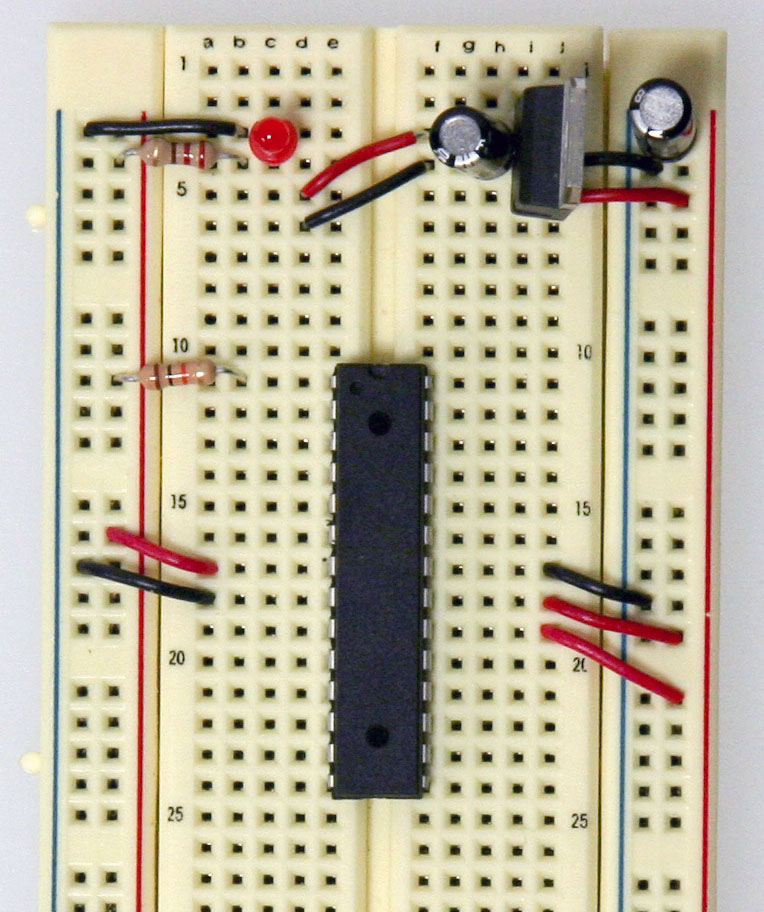
\includegraphics[scale=0.3]{img/arduino_breadboard/arduinobb_07.jpg}
 \caption{arduinobb 07}
 \label{arduinobb 07}
\end{figure}


\begin{figure}[!htb]
 \centering
 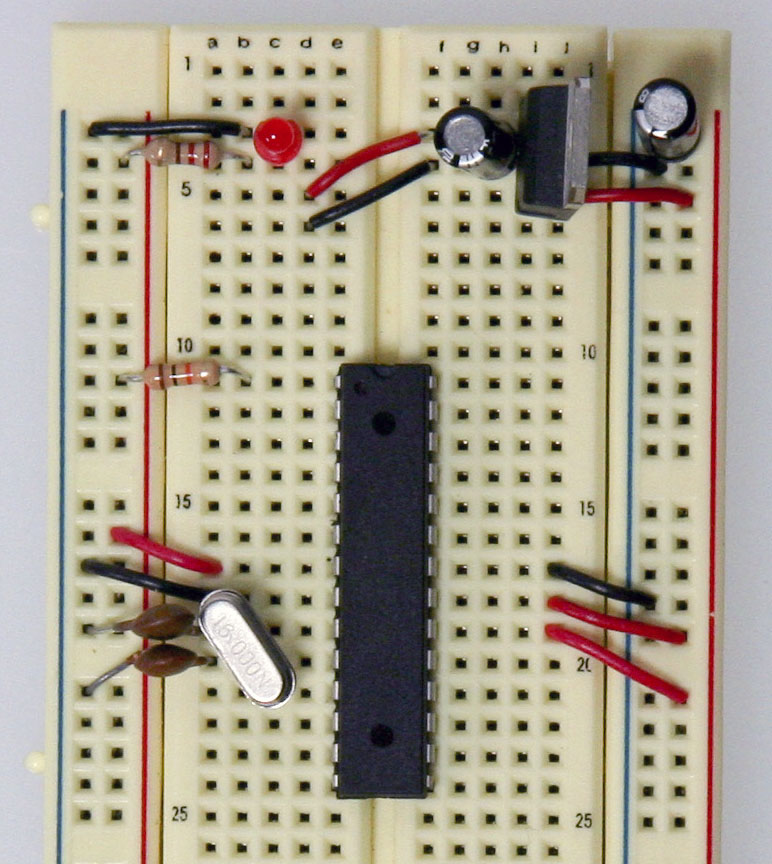
\includegraphics[scale=0.3]{img/arduino_breadboard/arduinobb_08.jpg}
 \caption{arduinobb 08}
 \label{arduinobb 08}
\end{figure}


\begin{figure}[!htb]
 \centering
 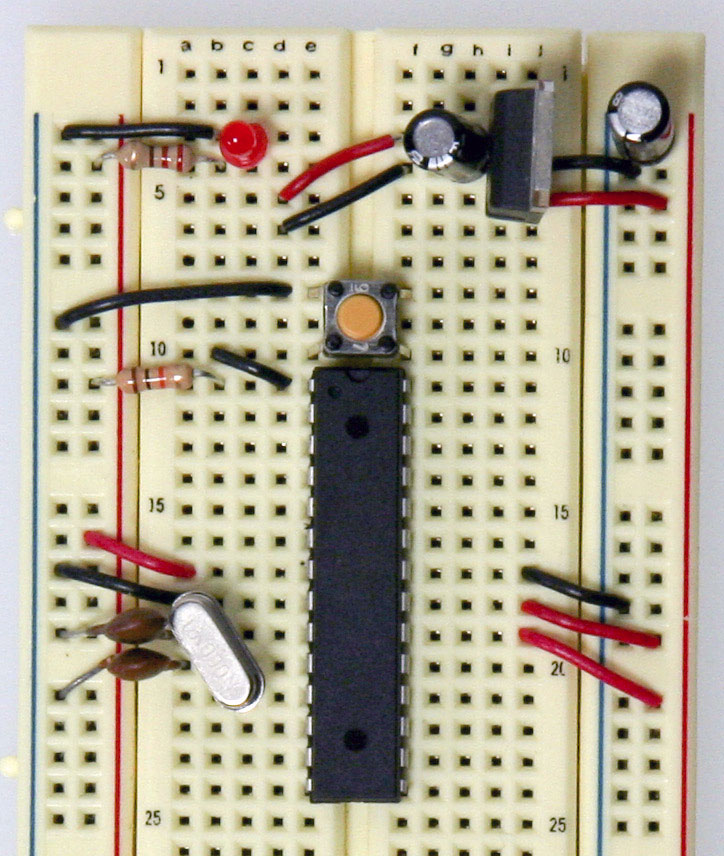
\includegraphics[scale=0.3]{img/arduino_breadboard/arduinobb_09.jpg}
 \caption{arduinobb 09}
 \label{arduinobb 09}
\end{figure}


\begin{figure}[!htb]
 \centering
 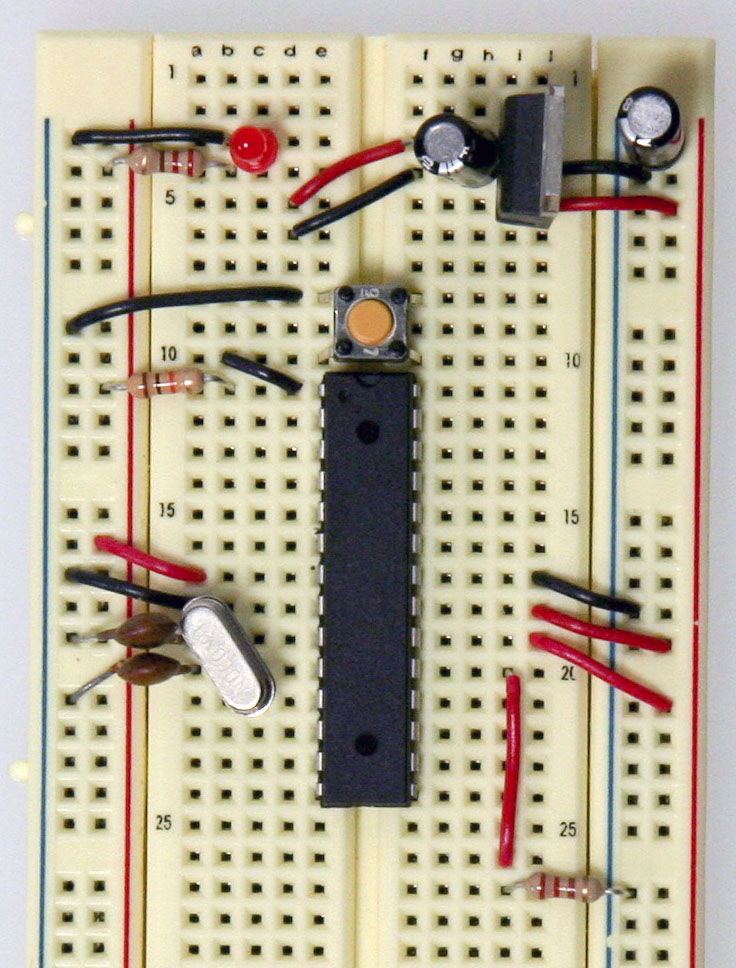
\includegraphics[scale=0.3]{img/arduino_breadboard/arduinobb_10.jpg}
 \caption{arduinobb 10}
 \label{arduinobb 10}
\end{figure}


\begin{figure}[!htb]
 \centering
 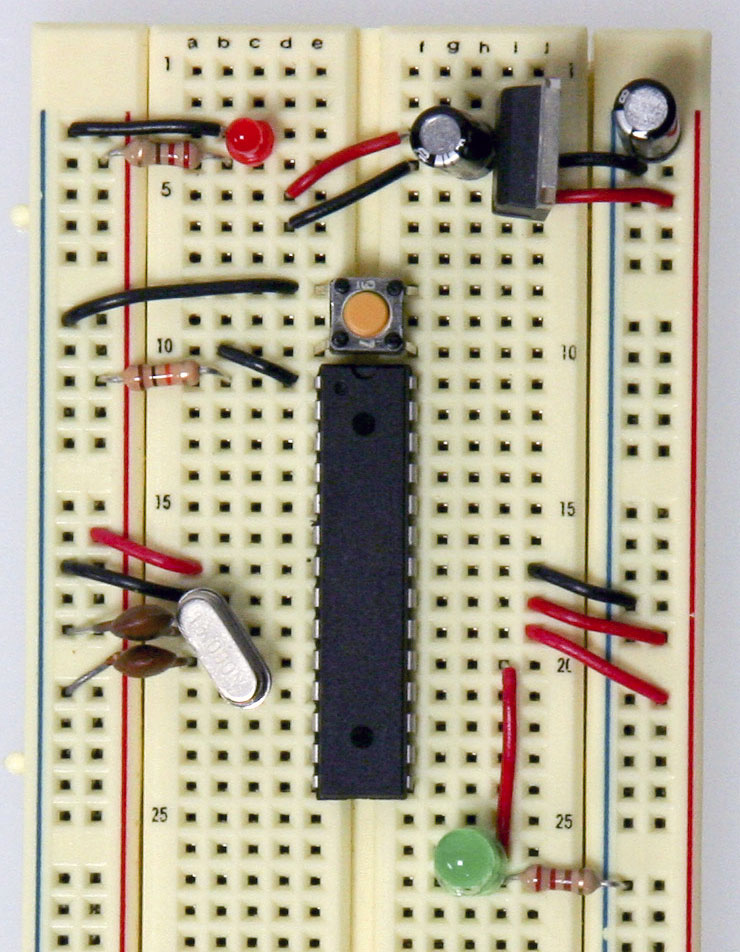
\includegraphics[scale=0.3]{img/arduino_breadboard/arduinobb_11.jpg}
 \caption{arduinobb 11}
 \label{arduinobb 11}
\end{figure}


\begin{figure}[!htb]
 \centering
 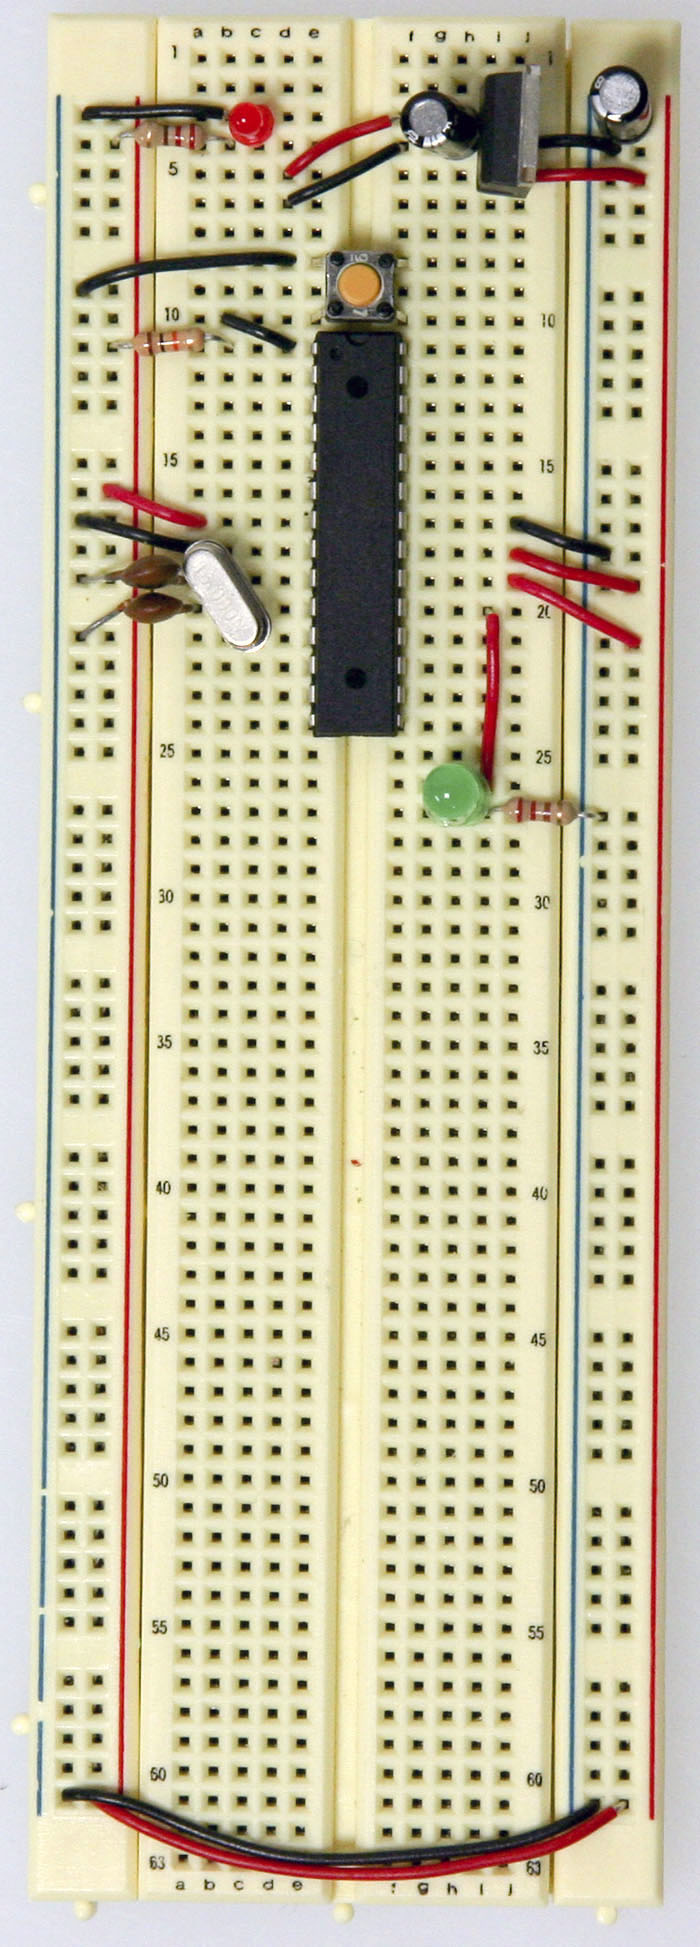
\includegraphics[scale=0.3]{img/arduino_breadboard/arduinobb_12.jpg}
 \caption{arduinobb 12}
 \label{arduinobb 12}
\end{figure}


\begin{figure}[!htb]
 \centering
 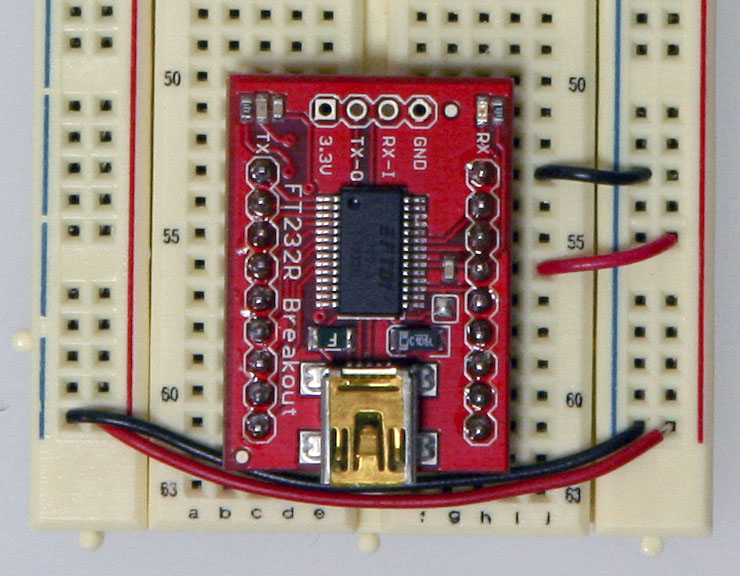
\includegraphics[scale=0.3]{img/arduino_breadboard/arduinobb_13.jpg}
 \caption{arduinobb 13}
 \label{arduinobb 13}
\end{figure}


\begin{figure}[!htb]
 \centering
 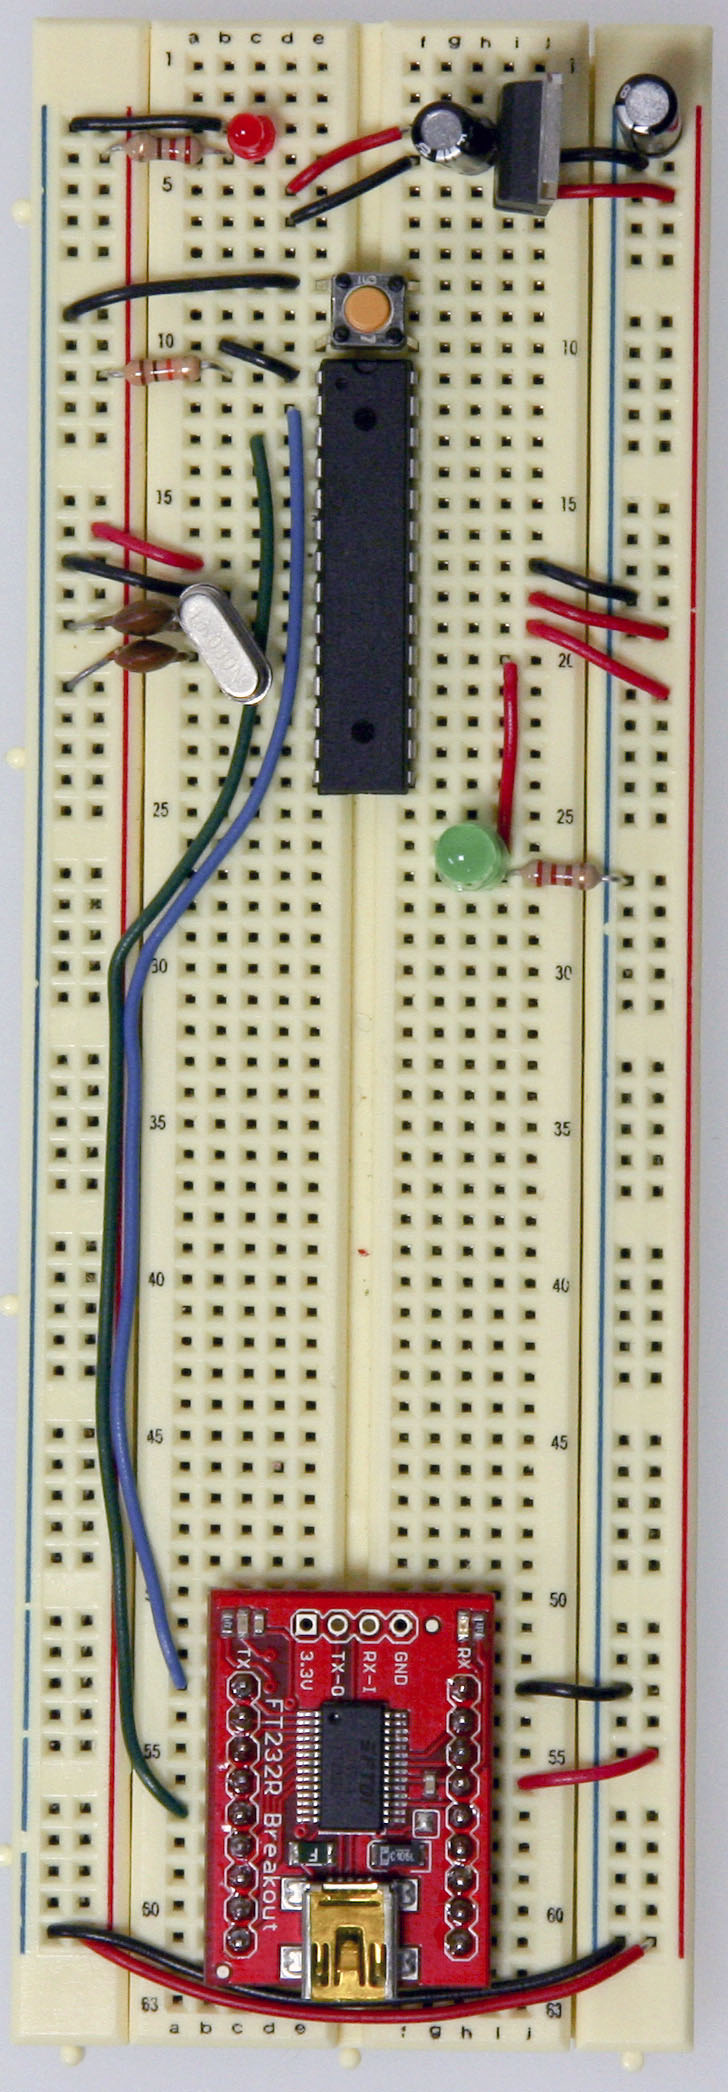
\includegraphics[scale=0.3]{img/arduino_breadboard/arduinobb_14.jpg}
 \caption{arduinobb 14}
 \label{arduinobb 14}
\end{figure}


\begin{figure}[!htb]
 \centering
 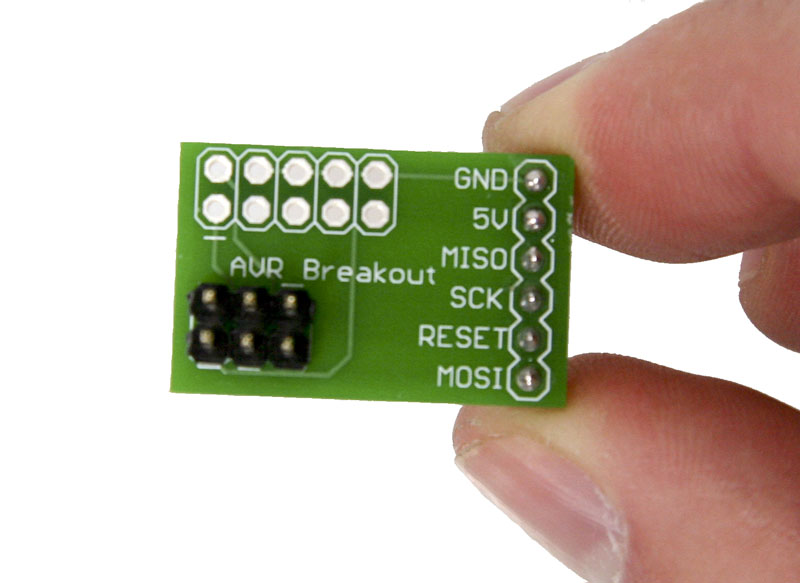
\includegraphics[scale=0.3]{img/arduino_breadboard/arduinobb_avradapter.jpg}
 \caption{arduinobb avradapter}
 \label{arduinobb avradapter}
\end{figure}


\begin{figure}[!htb]
 \centering
 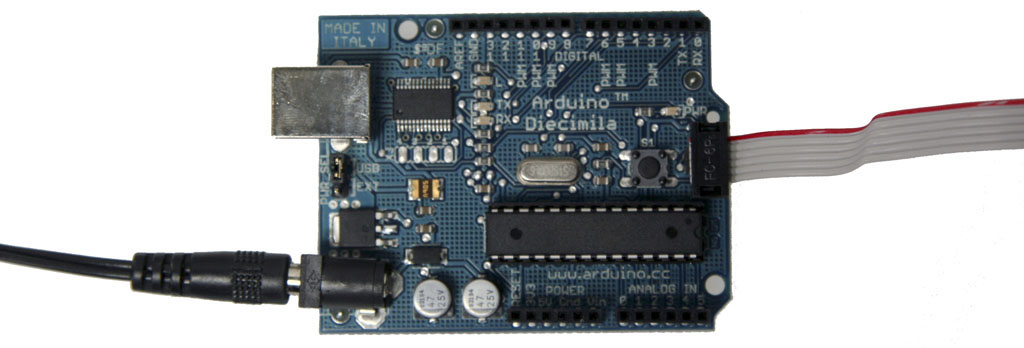
\includegraphics[scale=0.3]{img/arduino_breadboard/arduinobb_bootload1.jpg}
 \caption{arduinobb bootload1}
 \label{arduinobb bootload1}
\end{figure}


\begin{figure}[!htb]
 \centering
 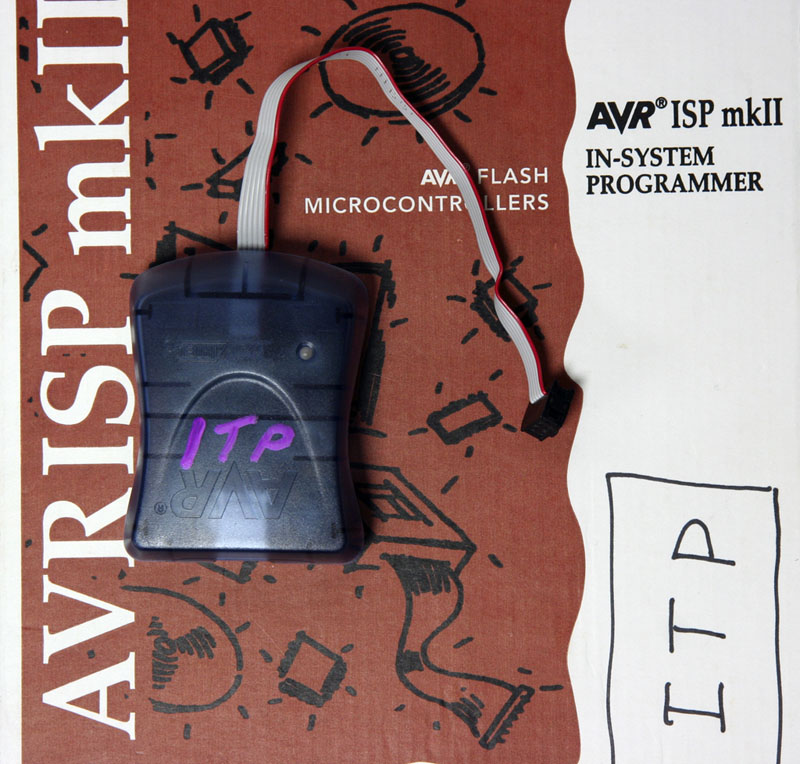
\includegraphics[scale=0.3]{img/arduino_breadboard/arduinobb_mk2.jpg}
 \caption{arduinobb mk2}
 \label{arduinobb mk2}
\end{figure}


\begin{figure}[!htb]
 \centering
 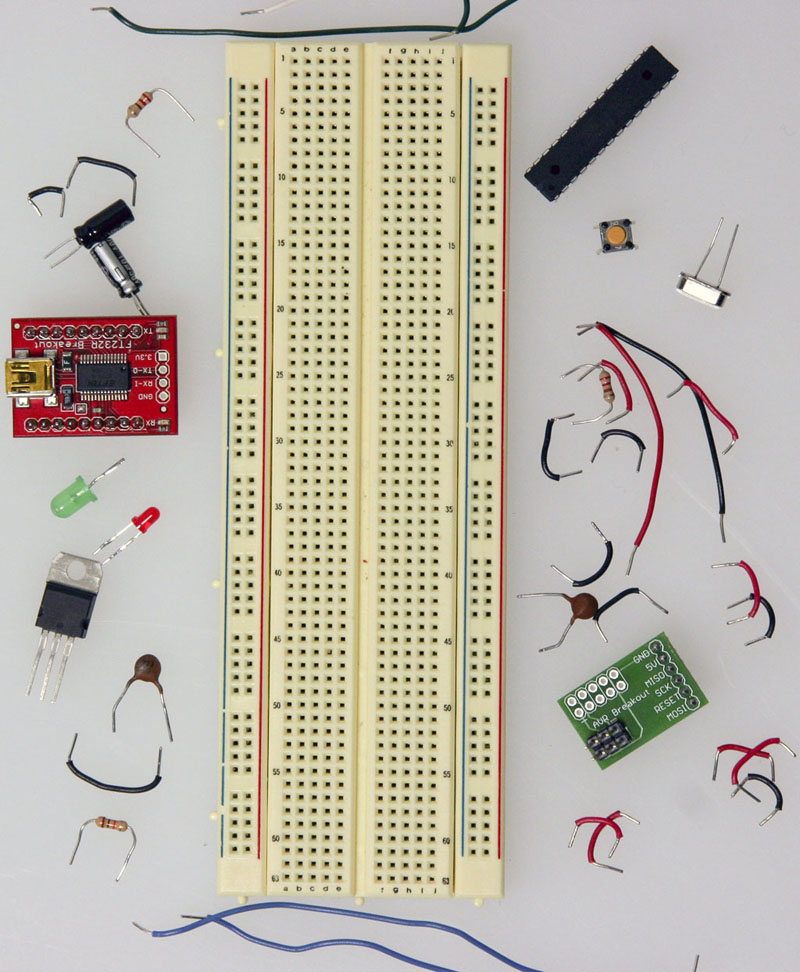
\includegraphics[scale=0.3]{img/arduino_breadboard/arduinobb_parts.jpg}
 \caption{arduinobb parts}
 \label{arduinobb parts}
\end{figure}


\begin{figure}[!htb]
 \centering
 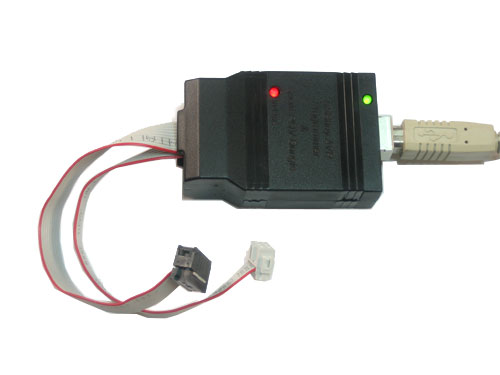
\includegraphics[scale=0.3]{img/arduino_breadboard/arduinobb_tiny.jpg}
 \caption{arduinobb tiny}
 \label{arduinobb tiny}
\end{figure}


\begin{figure}[!htb]
 \centering
 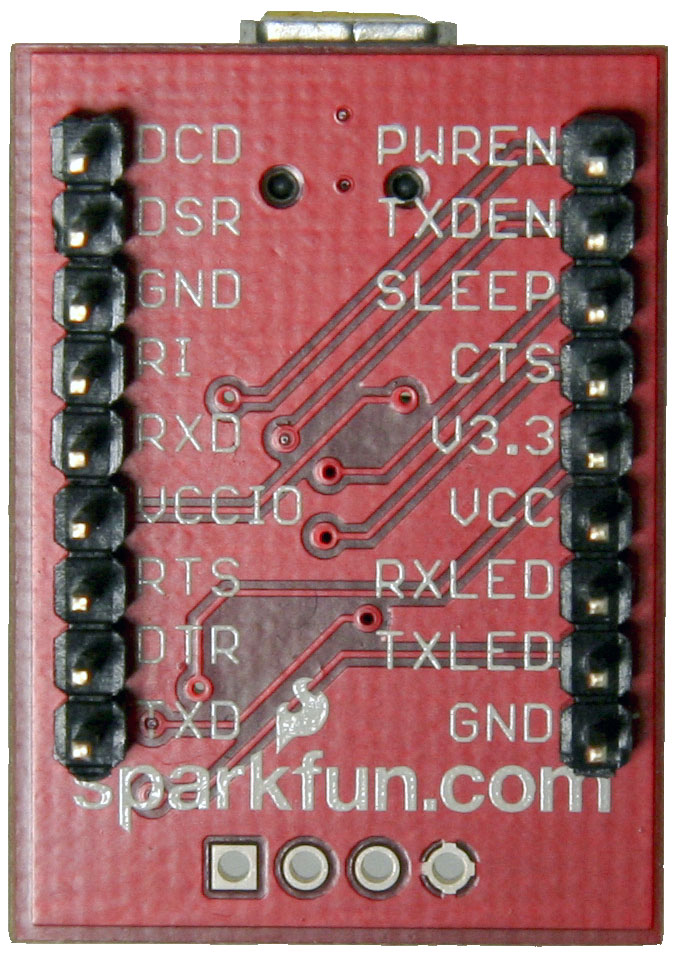
\includegraphics[scale=0.3]{img/arduino_breadboard/arduinobb_usbback.jpg}
 \caption{arduinobb usbback}
 \label{arduinobb usbback}
\end{figure}


\begin{figure}[!htb]
 \centering
 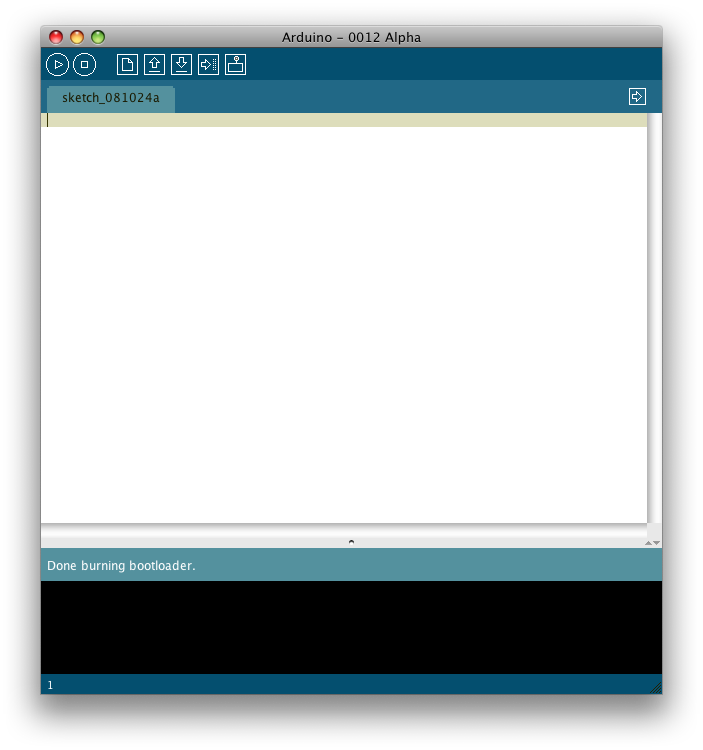
\includegraphics[scale=0.3]{img/arduino_breadboard/arduinobload_burndone.png}
 \caption{arduinobload burndone}
 \label{arduinobload burndone}
\end{figure}


\begin{figure}[!htb]
 \centering
 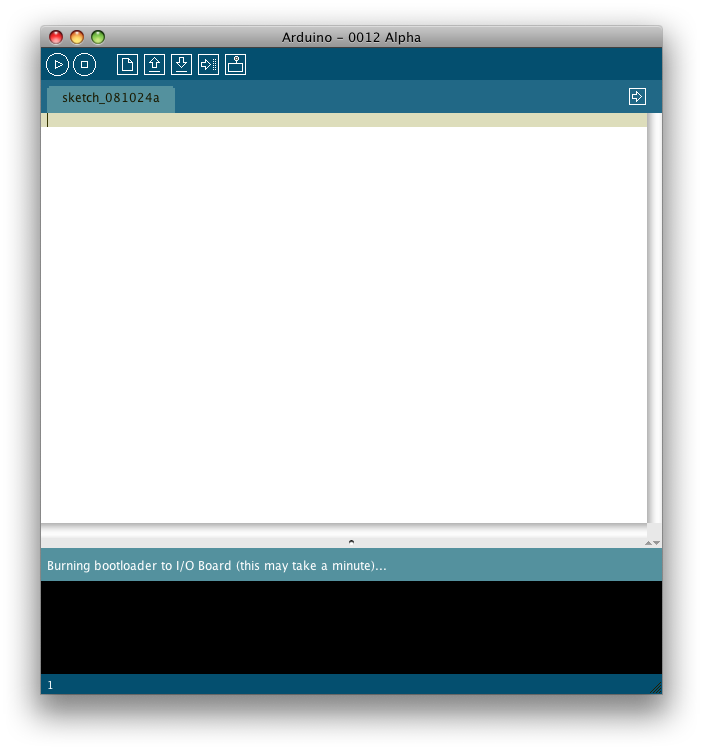
\includegraphics[scale=0.3]{img/arduino_breadboard/arduinobload_burning.png}
 \caption{arduinobload burning}
 \label{arduinobload burning}
\end{figure}


\begin{figure}[!htb]
 \centering
 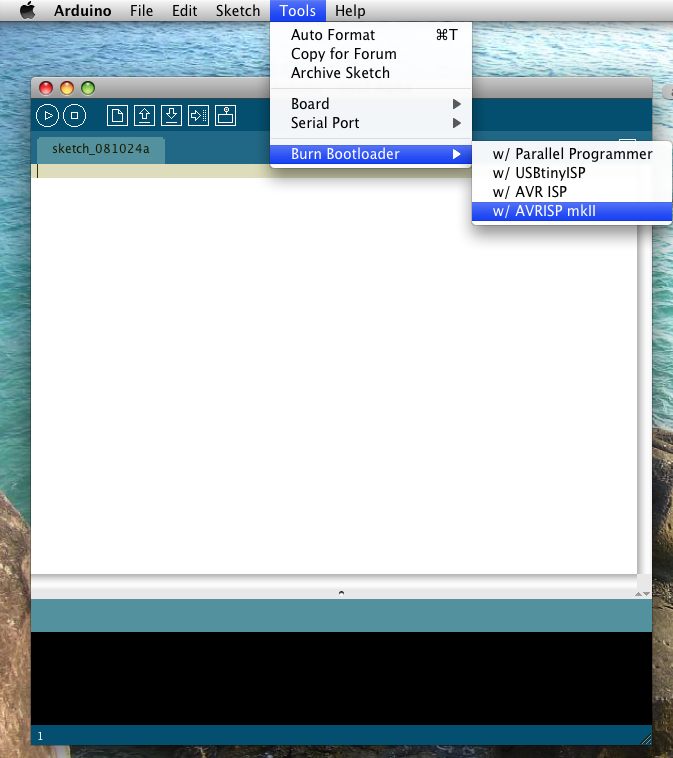
\includegraphics[scale=0.3]{img/arduino_breadboard/arduinobload_burn.png}
 \caption{arduinobload burn}
 \label{arduinobload burn}
\end{figure}


\begin{figure}[!htb]
 \centering
 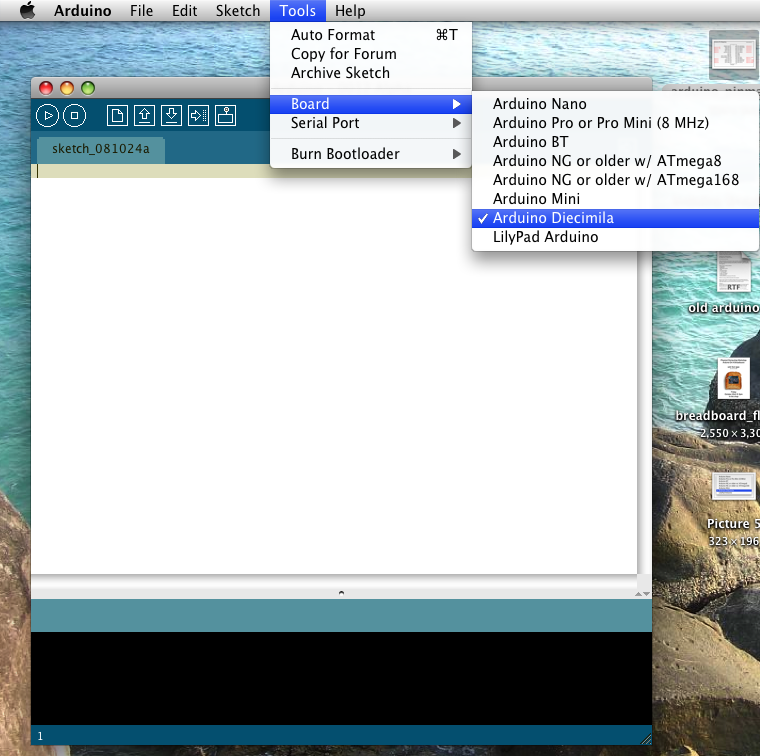
\includegraphics[scale=0.3]{img/arduino_breadboard/arduinobload_pickboard.png}
 \caption{arduinobload pickboard}
 \label{arduinobload pickboard}
\end{figure}


\begin{figure}[!htb]
 \centering
 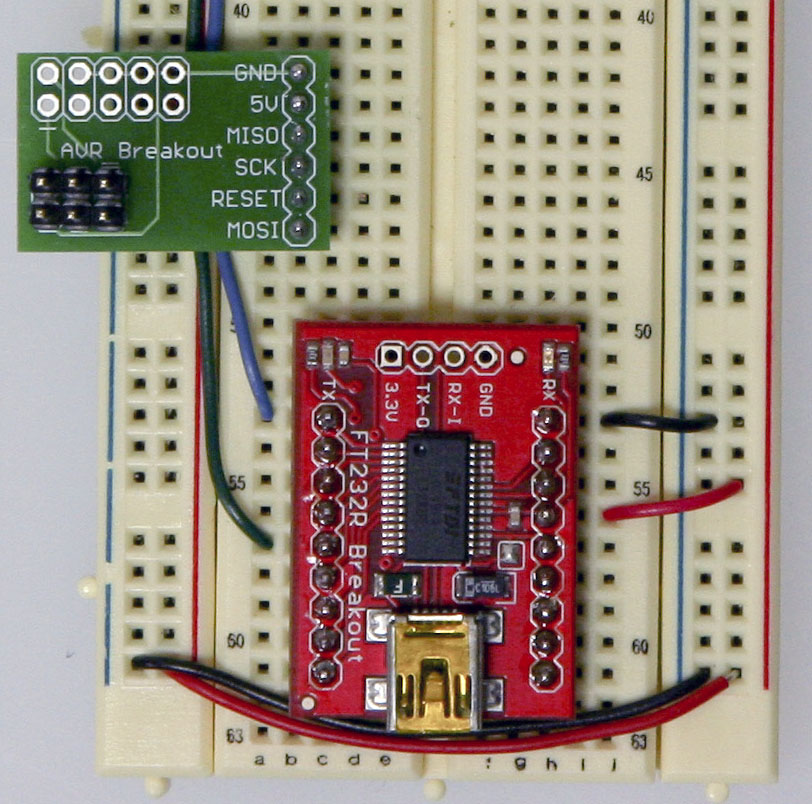
\includegraphics[scale=0.3]{img/arduino_breadboard/arduinobload_plugadapter.jpg}
 \caption{arduinobload plugadapter}
 \label{arduinobload plugadapter}
\end{figure}


\begin{figure}[!htb]
 \centering
 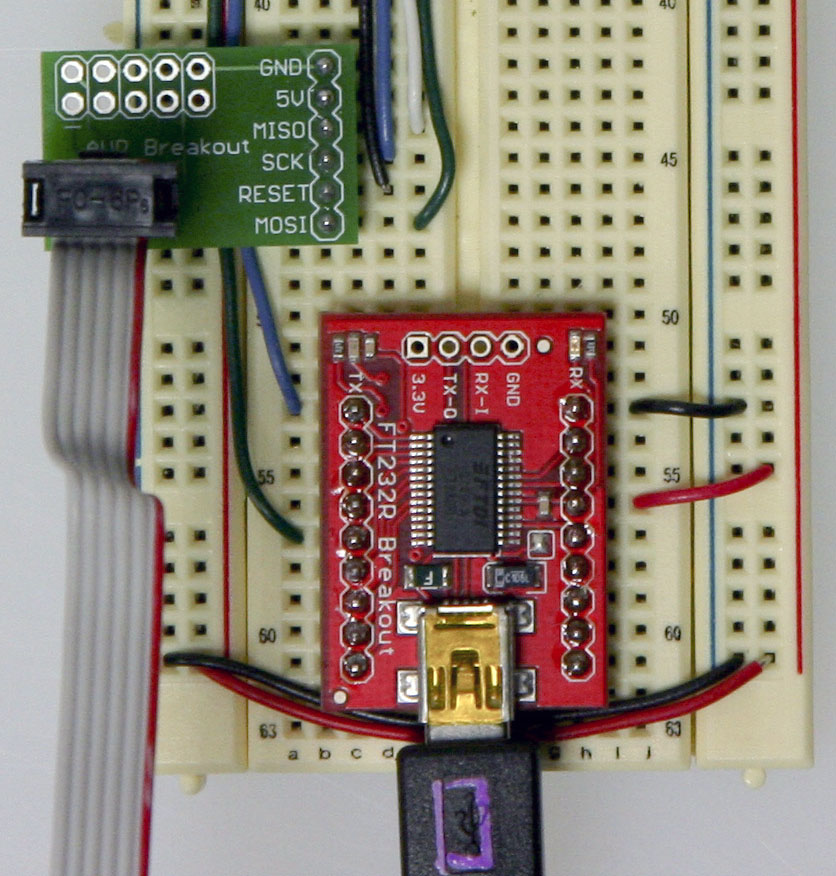
\includegraphics[scale=0.3]{img/arduino_breadboard/arduinobload_plugin.jpg}
 \caption{arduinobload plugin}
 \label{arduinobload plugin}
\end{figure}


\begin{figure}[!htb]
 \centering
 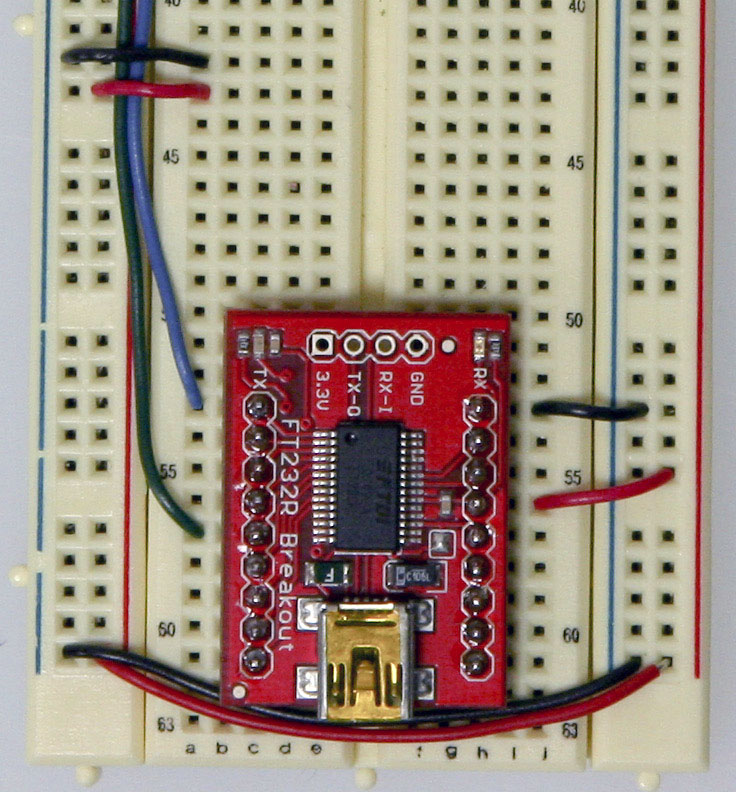
\includegraphics[scale=0.3]{img/arduino_breadboard/arduinobload_pwrgnd.jpg}
 \caption{arduinobload pwrgnd}
 \label{arduinobload pwrgnd}
\end{figure}


\begin{figure}[!htb]
 \centering
 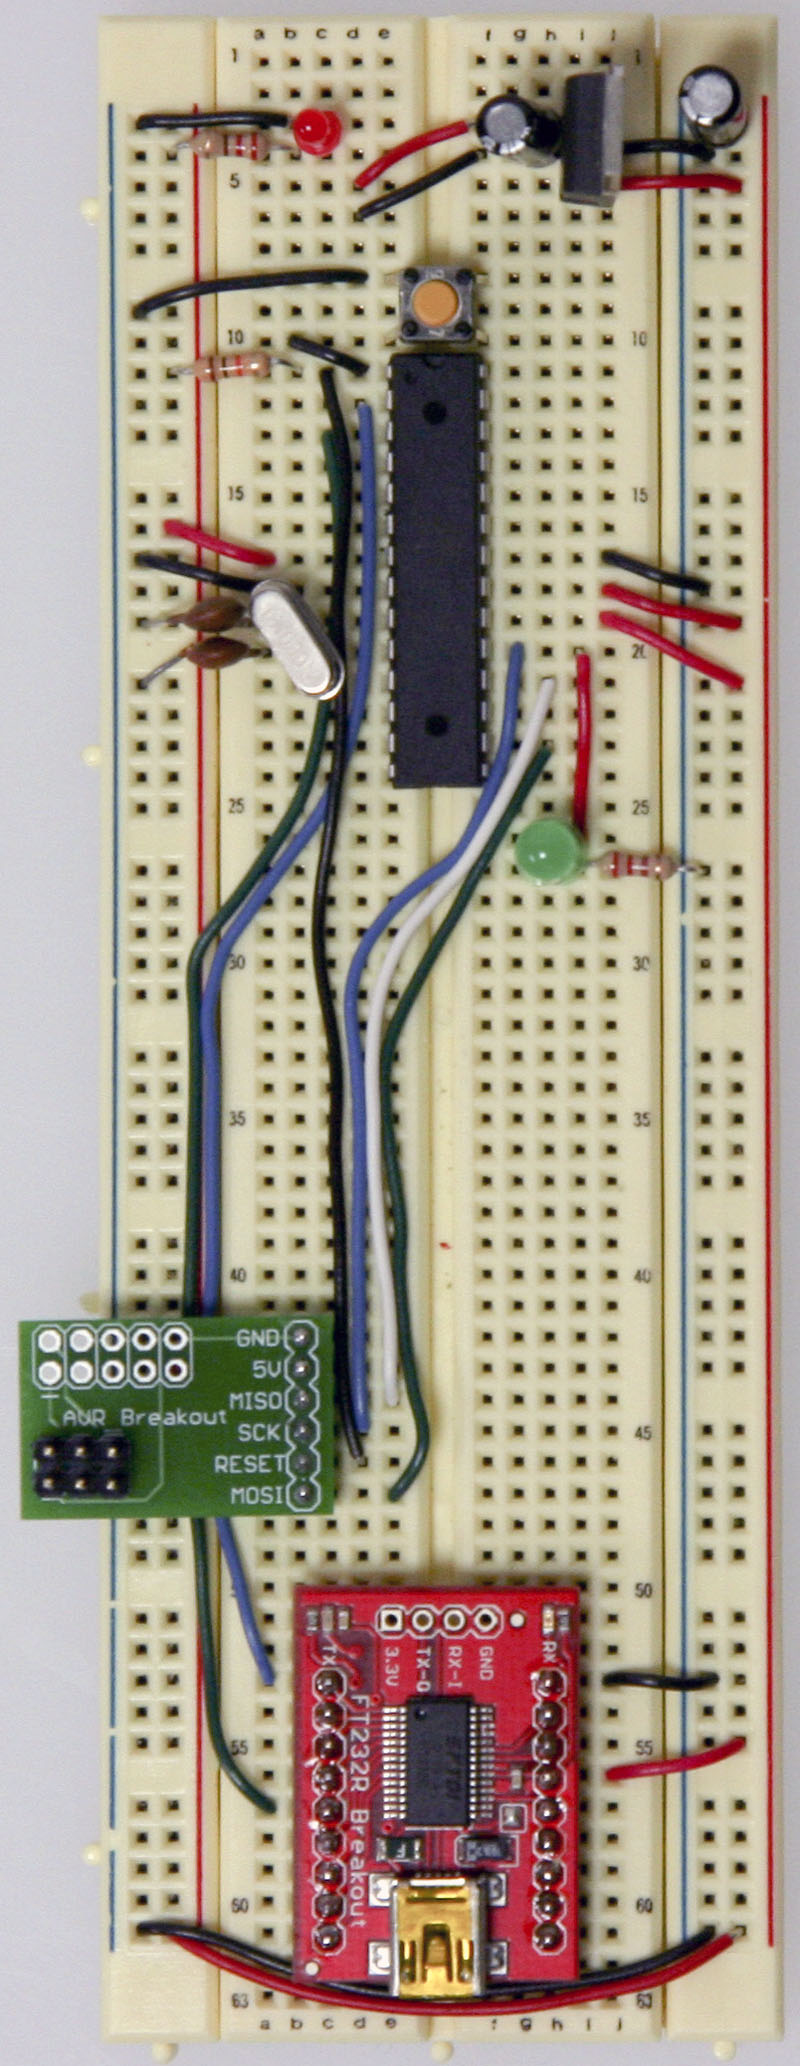
\includegraphics[scale=0.3]{img/arduino_breadboard/arduinobload_wires.jpg}
 \caption{arduinobload wires}
 \label{arduinobload wires}
\end{figure}


\begin{figure}[!htb]
 \centering
 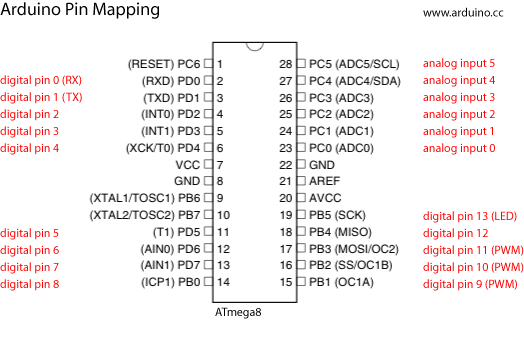
\includegraphics[scale=0.3]{img/arduino_breadboard/arduino_pinmap.png}
 \caption{arduino pinmap}
 \label{arduino pinmap}
\end{figure}


